	\section{Data Structures}
		\subsection{Weighted Union Disjoint Sets}
			\lstinputlisting{cpp/disjoint_sets.cpp}
		\subsection{BIT + Search}
			\lstinputlisting{cpp/binary_indexed_tree.cpp}
		\subsection{BIT Ranges}
			\lstinputlisting{cpp/BIT_ranges.cpp}
		\subsection{BIT 2D}
			\lstinputlisting{cpp/BIT_2d.cpp}
		\subsection{Segment Tree + Lazy Propagation}
			\lstinputlisting{cpp/segtree_lp.cpp}
		\subsection{Sparse Array}
			\lstinputlisting{cpp/sparse_array.cpp}
		\subsection{Monotonic Queue}
			\lstinputlisting{cpp/monotonic_queue.cpp}
		\subsection{Treap}
			\lstinputlisting{cpp/treap.cpp}
		\subsection{Skip Lists}
			\lstinputlisting{cpp/skip_lists.cpp}
	\section{Geometry}
		\subsection{Primitives}
			\lstinputlisting{cpp/2dprimitives.cpp}
		\subsection{Intersections}
			\lstinputlisting{cpp/2dintersections.cpp}
		\subsection{Rotations}
			\lstinputlisting{cpp/2drotation.cpp}
		\subsection{Minimum Enclosing Circle}
			\lstinputlisting{cpp/minimum_ec.cpp}
		\subsection{Triangle Area}
			\lstinputlisting{cpp/heron_triangle_area.cpp}
		\subsection{Polygon Cut}
			\lstinputlisting{cpp/polygon_cut.cpp}
		\subsection{Polygon Centroid + Area}
			\lstinputlisting{cpp/triangulation.cpp}
		\subsection{Point In Polygon}
			\lstinputlisting{cpp/point_in_poly.cpp}
		\subsection{Convex Hull}
			\lstinputlisting{cpp/convex_hull.cpp}
		\subsection{Line Segment Set Intersection}
			\lstinputlisting{cpp/line_segs_intersection.cpp}
		\subsection{Voronoi Diagrams}
			\lstinputlisting{cpp/voronoi.cpp}
		\subsection{Angular Sort}
			\lstinputlisting{cpp/angular_sort.cpp}
		\subsection{Line Sweep Closest Pair}
			\lstinputlisting{cpp/closest_pair.cpp}
		\subsection{Great Circle Distance}
			\lstinputlisting{cpp/great_circle_distance.cpp}
	\section{Combinatorics}
		\subsection{Basics}
			\lstinputlisting{cpp/combinatorics.cpp}
		\subsection{Permutation (Un)Ranking}
			\lstinputlisting{cpp/perm_ranking.cpp}
		\subsection{Combination (Un)Ranking}
			\lstinputlisting{cpp/comb_ranking.cpp}
	\section{Game Theory}
		\subsection{Nim Game}
			\lstinputlisting{cpp/nim_game.cpp}
		\subsection{Index-K Nim}
			\lstinputlisting{cpp/nim_game_k.cpp}
		\subsection{Greedy Nim}
			\lstinputlisting{cpp/nim_game_greedy.cpp}
		\subsection{Grundy Numbers}
			\lstinputlisting{cpp/grundy_numbers.cpp}
		\subsection{General Josephus Problem}
			\lstinputlisting{cpp/josephus.cpp}
	\section{Mathematics}
		\subsection{Inclusion-Exclusion Patterns}
			\lstinputlisting{cpp/inclusion_exclusion.cpp}
		\subsection{Determinant}
			\lstinputlisting{cpp/determinant.cpp}
		\subsection{Gaussian Elimination}
			\lstinputlisting{cpp/gaussian_elimination.cpp}
		\subsection{Fast Fourier-Transform}
			\lstinputlisting{cpp/fast_fourier.cpp}
		\subsection{Linear Programming Simplex}
			\lstinputlisting{cpp/simplex_tableau.cpp}
		\subsection{Continued Fractions of Rationals}
			\lstinputlisting{cpp/continued_fractions.cpp}
		\subsection{Tortoise \& Hare}
			\lstinputlisting{cpp/tortoise_hare.cpp}
		\subsection{Pollard Rho}
			\lstinputlisting[language=Java]{java/PollardRho.java}
		\subsection{Matrix Exponentiation}
			\lstinputlisting{cpp/fibosum.cpp}
	\section{Number Theory}
		\subsection{Extended GCD}
			\lstinputlisting{cpp/extended_gcd.cpp}
		\subsection{Modular Inverse}
			\lstinputlisting{cpp/modular_inverse.cpp}
		\subsection{Modular Linear Equation}
			\lstinputlisting{cpp/mod_linear_eqn.cpp}
		\subsection{Linear Diophantine Equation}
			\lstinputlisting{cpp/linear_diophantine.cpp}
		\subsection{Sieve of Eratosthenes}
			\lstinputlisting{cpp/sieve.cpp}
		\subsection{Primality Testing \& Factoring}
			\lstinputlisting{cpp/prime_factoring.cpp}
		\subsection{Euler Phi}
			\lstinputlisting{cpp/euler_phi.cpp}
		\subsection{Chinese Remainder}
			\lstinputlisting{cpp/chinese_remainder.cpp}
		\subsection{General Chinese Remainder}
			\lstinputlisting{cpp/chinese_general.cpp}
		\subsection{Discerete Logarithm}
			\lstinputlisting{cpp/discrete_log.cpp}
	\section{Graph Theory}
		\subsection{Articulation Points \& Bridges}
			\lstinputlisting{cpp/artpb.cpp}
		\subsection{SCC}
			\lstinputlisting{cpp/scc.cpp}
		\subsection{2-SAT}
			\lstinputlisting{cpp/2sat.cpp}
		\subsection{Edmonds-Karp Max Flow}
			\lstinputlisting{cpp/max_flow_edmond.cpp}
		\subsection{Dinic's Max Flow}
			\lstinputlisting{cpp/max_flow_dinic.cpp}
		\subsection{Min-Cost Max Flow}
			\lstinputlisting{cpp/min_cost_max_flow.cpp}
		\subsection{Euler Cycles}
			\lstinputlisting{cpp/euler_cycles.cpp}
		\subsection{Maximum Matching}
			\lstinputlisting{cpp/max_bp_matching.cpp}
		\subsection{HL Decomposition}
			\lstinputlisting{cpp/hl_decomposition.cpp}
		\subsection{Modelling Inequalities}
			\lstinputlisting{cpp/modeling_inequalities.cpp}
		\subsection{Bellman Ford}
			\lstinputlisting{cpp/bellman_ford.cpp}
		\subsection{Stable Marriage}
			\lstinputlisting{cpp/stable_marriage.cpp}
	\section{Strings}
		\subsection{Aho Corasick}
			\lstinputlisting{cpp/aho.cpp}
		\subsection{Hashing}
			\lstinputlisting{cpp/hashing.cpp}
		\subsection{Z-Algorithm}
			\lstinputlisting{cpp/zalgo.cpp}
		\subsection{KMP}
			\lstinputlisting{cpp/kmp.cpp}
		\subsection{Manacher}
			\lstinputlisting{cpp/manacher.cpp}
		\subsection{Palindromic Tree}
			\lstinputlisting{cpp/palindromic_tree.cpp}
		\subsection{Suffix Array \& LCP}
			\lstinputlisting{cpp/suffix_array.cpp}
		\subsection{Trie}
			\lstinputlisting{cpp/trie.cpp}
		\subsection{Chomsky Normal Form}
			\lstinputlisting{cpp/chomsky.cpp}
		\subsection{CYK}
			\lstinputlisting{cpp/cyk.cpp}
	\section{Misc}
		\subsection{Binary Search}
			\lstinputlisting{cpp/binary_search.cpp}
		\subsection{Ternary Search}
			\lstinputlisting{cpp/ternary_search.cpp}
		\subsection{Sqrt Decomposition}
			\lstinputlisting{cpp/sqrt_decomposition.cpp}
		\subsection{Rhombus Matrix Rotation}
			\lstinputlisting{cpp/diamond_rot.cpp}
		\subsection{Lower Envelope}
			\lstinputlisting{cpp/lower_envelope.cpp}
	\section{Theoretical References}
		\includepdf[pages={2-4, 7-11},nup=2x2, delta = -35 -55,offset = 0 -5,pagecommand={\pagestyle{fancy}}]{others/saratov_lib}